
\documentclass[12pt]{article}
\usepackage[a4paper, margin=.30in]{geometry}
\usepackage{graphicx ,
            wrapfig,
            xcolor, 
            enumerate,
            amsmath,
			fontenc,
			tcolorbox,circuitikz,tikz,bm
            }
			\usepackage{pgfplots}
\pgfplotsset{compat=newest}
\usepgfplotslibrary{fillbetween}
\usepackage{pgfplots}
\newcommand\headerMe[2]{\noindent{}#1\hfill#2}
\renewcommand{\thesection}{\Roman{section}}

\author{Zakaria HAOUZAN}
\date{\today}

\begin{document}
% headers --------------
\headerMe{Matière : Physique-Chimie}{Professeur : Zakaria HAOUZAN}\\
\headerMe{Unité : Mécanique }{Établissement : Lycée SKHOR qualifiant}\\
\headerMe{Niveau : 2BAC-SM-PC}{Heure : 5H}\\

% ------Content ________
\begin{center}

    \Large{Leçon $N^{\circ} 16 $: \color{red}Aspects énergétiques}
\end{center}


\section{Travail de la tension d'un ressort : }
\subsection{Travail d'une force constante lors d'un déplacement rectiligne:}



Le Travail d'une force constante entre deux points A et B est égale au produit scalaire du vecteur force $\vec{F}$ par le vecteur déplacement $\vec{AB}$ : $$W_{A\rightarrow B}(\vec{F}) = \vec{F}.\vec{AB} =F.AB.cos(F.AB)$$

\subsection{Travail de la tension d'un ressort:}
Considérons un ressort de longueur initiale $l_0$ et de constante de raideur K placé sur un plan horizontal comme l'indique la figure : 


\begin{wrapfigure}{r}{0.3\textwidth}
\begin{center}
	\vspace{-1.7cm}
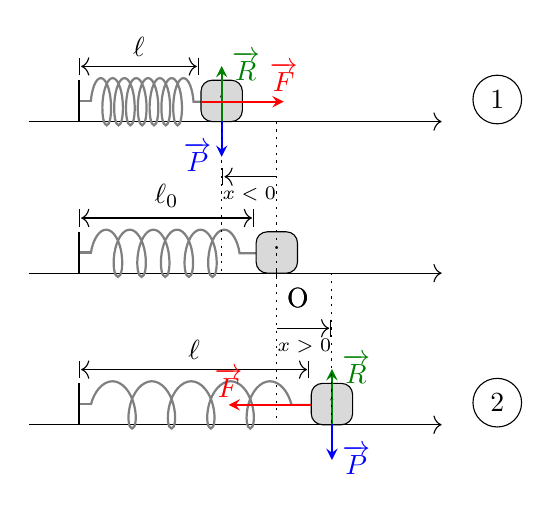
\begin{tikzpicture}[scale=0.7]
	
\tikzset{ressort/.style={thick,gray,smooth}} %définition d'un style de ressort
	\usetikzlibrary{patterns}
\coordinate (O) at (0,-2.75); 
	\draw [->] (-4.5,-2.75) -- (3,-2.75) ;
\begin{scope}[shift=({0,-2.75})]     

	\begin{scope}[scale=0.75,shift=({-4.78,0.5}),rotate around={90:(0,0)}]
	  %bloc qui tient le ressort

		\draw[thick,gray] (0,0) -- (0,-0.3); 
		%\fill [pattern=north east lines] (-0.5,0) rectangle (0.5,0.3); 
		\draw[thick](-0.5,0)--(0.5,0);
		%fin ressort       
	\end{scope}
	 \draw [ressort,decorate,decoration={coil,aspect=0.4,segment length=3mm,amplitude=3mm}] (-3.375,0.36)--++(3,0) ;
	 \draw[rounded corners=4pt,fill=gray!30] (-0.375,0) rectangle++ (0.75,0.75) node [midway, shift=({0,0.05})] {$.$};  
 %repérage de \ell
	\draw [|<->|] (-3.6,1) -- (-0.4,1) node [midway,above] {$\ell_0$}; 
\end{scope}

%--------------------FIN ressort central---------------------	


	%----------ressort comprimé------------
	\coordinate (M) at (-1,0.36);
	\draw (O) --++ (0,0.1) (O) --++ (0,-0.1) node [below right] {O}; 
    
	\node[draw, circle] at (4,0.4) {1};  

	%Axe
	\draw [->] (-4.5,0) -- (3,0) ;  

	%repérage de x
	\draw [|<-] (-1,-1) -- (0,-1) node [midway,below] {\scriptsize  $x<0$};

	%repérage de \ell
	\draw [|<->|] (-3.6,1) -- (-1.4,1) node [midway,above] {$\ell$};

	\begin{scope}[scale=0.75,shift=({-4.78,0.5}),rotate around={90:(0,0)}]
	  %bloc qui tient le ressort
		\draw[thick,gray] (0,0) -- (0,-0.3); 
		\draw[thick](-0.5,0)--(0.5,0);
		%fin ressort       
	\end{scope}	   

	%ressort  
	\draw [ressort,decorate,decoration={coil,aspect=0.3,segment length=1.5mm,amplitude=3mm}] (-3.375,0.36)--++(2,0) ;
	\draw[rounded corners=4pt,fill=gray!30] (-1.375,0) rectangle++ (0.75,0.75) node [midway, shift=({0,0.05})] {$.$}; 

	\draw [->,-stealth,thick,blue] (M) --++(0,-1) node [left] {$\overrightarrow{P}$};   
	\draw [->,-stealth,thick,green!50!black] (M)++(0,-0.35) --++(0,+1) node [right] {$\overrightarrow{R}$};   
	\draw [->,-stealth,thick,red] (M)++(-0.375,0)--++(1.5,0) node [above] {$\overrightarrow{F}$};     
	%----------FIN ressort comprimé------------ 

%----------ressort etiré------------

	\begin{scope}[shift=({0,-5.5})]

	\coordinate (M) at (1,0.36);
	\draw (O) --++ (0,0.1) (O) --++ (0,-0.1) node [below right] {O}; 
     
	\node[draw, circle] at (4,0.4) {2};
   

	%Axe
	\draw [->] (-4.5,0) -- (3,0) ;  

	%repérage de x
	\draw [->|] (0,1.75) -- (1,1.75) node [midway,below] {\scriptsize $x>0$};

	%repérage de \ell
	\draw [|<->|] (-3.6,1) -- (0.6,1) node [midway,above] {$\ell$};

	\begin{scope}[scale=0.75,shift=({-4.78,0.5}),rotate around={90:(0,0)}]
	  %bloc qui tient le ressort
		\draw[thick,gray] (0,0) -- (0,-0.3); 
		\draw[thick](-0.5,0)--(0.5,0);
		%fin ressort       
	\end{scope}	   

	%ressort  
	\draw [ressort,decorate,decoration={coil,aspect=0.5,segment length=5mm,amplitude=3mm}] (-3.375,0.36)--++(4,0) ; 

	 \draw[rounded corners=4pt,fill=gray!30] (0.625,0) rectangle++ (0.75,0.75) node [midway, shift=({0,0.05})] {$.$}; 

	\draw [->,-stealth,thick,blue] (M) --++(0,-1) node [right] {$\overrightarrow{P}$};   
	\draw [->,-stealth,thick,green!50!black] (M)++(0,-0.35) --++(0,+1) node [right] {$\overrightarrow{R}$};   
	\draw [->,-stealth,thick,red] (M)++(-0.375,0)--++(-1.5,0) node [above=-1] {$\overrightarrow{F}$};	


	\end{scope}    

	\draw [dotted] (-1,0) --++(0,-2.75);  
	\draw [dotted] (1,-2.75) --++(0,-2.75);  
	\draw [dotted] (0,0) --++(0,-5.5);  

\end{tikzpicture}

\end{center}
\end{wrapfigure}
La tension du ressort $\vec{T} = -K.x.\vec{i}$ n'est pas une force constante.

Pour Calculer le Travail de cette force on doit Considerer le travail élémentaire de cette force $\delta{W}$ sur un déplacement infiniment petit $\delta{\vec{l}}$ sur lequel nous Considérons que la force est constante $\delta{W} =  \vec{T}.\delta{\vec{l}}$ avec $\delta{\vec{l}}$=$\delta{x}.\vec{i}$.

donc : $\delta{W} = \vec{F}.\delta{\vec{l}} = -K.x.\vec{i}.\delta{x}.\vec{i} = -K.x\delta{x} $ 

Le travail total de la tension $\vec{T}$ du ressort lorsque son point d'application se déplace d'un point
d'abscisse $x_1$ à un point d'abscisse $x_2$ est la somme des travaux élémentaire , on obtient : 

$$dW = -Kx.dx$$
donc $$ W_{A \rightarrow B}(\vec{T})   = \int_{x_1}^{x_2} -K.x.\,\mathrm{d}x = -K\int_{x_1}^{x_2} x.\,\mathrm{d}x
$$

alors :$$ W_{A \rightarrow B}(\vec{T})= K.\big[ \frac{x^2}{2}\big]_{x_1}^{x_2}$$ 

Donc le travail de la tension du ressort lorsque son point d'application se déplace d'un point M1d'abscisse $x_1$ à un point $M_2$ 

d'abscisse x2 est donné par la relation suivante $ W_{A \rightarrow B}(\vec{T}) = \frac{1}{2}.K.(x_1^2 - x_2^2) $


\section{Etude énergétique du pendule élastique :}

\subsection{Energie potentielle de élastique:}

L'énergie potentielle élastique d'un pendule élastique est l'énergie qu'il possède grâce à la déformation du ressort, elle est donnée par la relation suivante:  $E_{pe} = \frac{1}{2}.K.x^2 + C$

C: est une constante qui dépend du choix de l’état de référence de l’énergie potentielle élastique .

x : allongement du ressort (en mètre)

$E_{pe}$: énergie potentielle élastique en (J).

En considérant comme état de référence $E_{pe} = 0$ lorsque x = 0 La constante C=0 donc $E_{pe} = \frac{1}{2}.K.x^2$

\begin{tcolorbox}
Remarque : La variation de l'énergie potentielle ne dépend pas de l'état de référence . En effet 

- dans la position $x_1$ On a $E_{pe1} = \frac{1}{2}.K.x_1 + C$


- dans la position $x_2$ On a $E_{pe2} = \frac{1}{2}.K.x_2 + C$

- La variation de l’énergie potentielle $\Delta{E_p}=E_{p2}-E_{p1} = \frac{1}{2}.K.\big(x_2^2 - x_1^2\big)$

- donc $W_{A \rightarrow B}(\vec{T}) = - \Delta{E_p}$
\end{tcolorbox}

\subsection{Conservation de l'énergie mécanique:}
Pendant les oscillations libres non amorties d'un pendule élastique horizontal constitué d'un corps S de masse m et d'un
ressort de constante de raideur K. 





appliquons le théorème de l'énergie cinétique sur le corps S entre un point M1d'abscisse $x_1$ à
d'abscisse $x_2$ un point $M_2$ : $\Delta_{1 \rightarrow 2}{Ec} = W_{1 \rightarrow 2}(\vec{P}) +  W_{1 \rightarrow 2}(\vec{R}) + W_{1 \rightarrow 2}(\vec{T})$

On a $W(\vec{P})_{1 \rightarrow 2} =W(\vec{R})_{1 \rightarrow 2}= 0$

donc $\Delta{Ec}_{1 \rightarrow 2} = W(\vec{T})_{1 \rightarrow 2}$ or $\Delta{Epe}_{1 \rightarrow 2} =- W(\vec{T})_{1 \rightarrow 2}$

alors $\Delta{E_m} = 0$  donc $E_{m1} = E_{m2}$ donc l'énergie mécanique est constante.

\subsection{Détermination de l'équation différentielle par étude énergétique: }

Si les frottement sont négligeables , l'énergie mécanique de l'oscillateur est constante $E_m = Constante$ donc $\frac{dE_m}{dt} = 0$

Or $Em = Ec + Ep = \frac{1}{2}.m\dot{x} + \frac{1}{2}.K.x^2$

d’où l'équation différentielle: $m.\ddot{x} + K.x = 0$

\subsection{Expression de l'énergie mécanique du pendule élastique:}

La solution de l'équation différentielle: $m.\ddot{x}+K.x=0$ est $x_m.\cos(\frac{2.\pi}{T_0}.t + \phi)$ avec $T_0 = 2.\pi.\sqrt{\frac{m}{K}}$

avec $v = \dot{x} = -x_m.\frac{2.\pi}{T_0}.sin(\frac{2.\pi}{T_0}.t+\phi)$

$E_m = E_p + E_c = \frac{1}{2}K.x_m^2$

\subsection{Diagramme énergétiques : }
\subsubsection{Cas des oscillations sans frottements :}
Dans le cas des oscillations sans frottements l'énergie mécanique de l'oscillateur mécanique est constante. $$E_m = \frac{1}{2}.K.x_m^2 = \frac{1}{2}.m.v_{max}^2 = C^{te}$$


En considérant comme état de référence Epe=0 lorsque x=0 on a C=0 donc : $E_{pe} = \frac{1}{2}.K.x^2$

En représentant la variation Epe ,Ec et Em en fonction de x on obtient le diagramme suivant: 

A chaque instant on a ; Em=EC+Epe donc : Ec=Em-Epe
Et en représentant la variation de Epe ,Ec et Em en fonction du temps on obtient le diagramme suivant:

\begin{center}
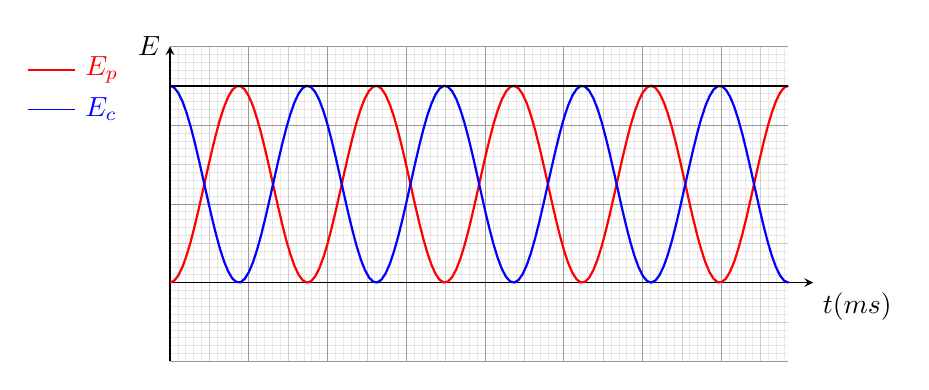
\begin{tikzpicture}[scale=1]
%papier milli
\draw [very thin, gray!20] (0,-1) grid[step=0.1] (2.5*pi,3);
\draw [very thin, black!20] (0,-1) grid[step=0.5] (2.5*pi,3);
\draw [very thin, black!40] (0,-1) grid[step=1] (2.5*pi,3);
%fin 
axes \draw[->,>=stealth] (0,0) -- (2.6*pi,0) node[below right] {$t (ms)$};
%stealth définit un style de flèche, "furtif"
\draw[->,>=stealth] (0,-1) -- (0,3) node[left] {$E$};
%\draw (1,0.1) -- (1,-0.1) node [below right] {{\scriptsize $0.2$}}; %échelle abscisse
%\draw (0.1,1) -- (-0.1,1) node [left] {{\scriptsize $2V$}}; %échelle ordonnée
%fin
%legende \draw (-2,3) -- (-0.4,3) -- (-0.4,1.9) -- (-2,1.9) -- (-2,3); %cadre
\draw [red] (-1.8,2.7)--(-1.2,2.7) node [right] [red] {$E_p$};
\draw [blue] (-1.8,2.2)--(-1.2,2.2) node [right] [blue] {$E_c$};
%fin
\draw[color=red,thick,domain=0:2.5*pi, samples=150] plot ({\x},{2.5*sin(1.8*\x r )^2});
\draw[color=blue,thick,domain=0:2.5*pi, samples=150] plot ({\x},{2.5*cos(1.8*\x r )^2});

\draw[color=black,thick,domain=0:2.5*pi, samples=150] plot ({\x},{2.5});
\end{tikzpicture}

\end{center}


\begin{center}
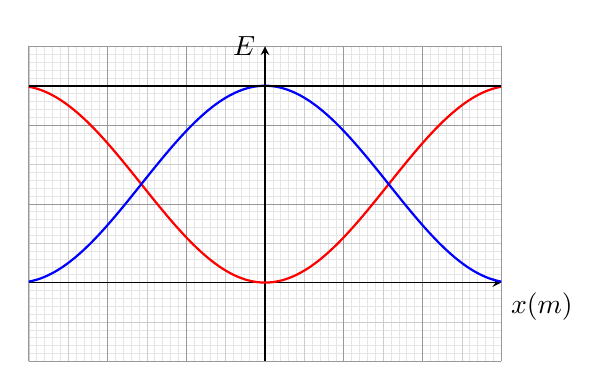
\begin{tikzpicture}[scale=1]
%papier milli
\draw [very thin, gray!20] (-3,-1) grid[step=0.1] (3,3);
\draw [very thin, black!20] (-3,-1) grid[step=0.5] (3,3);
\draw [very thin, black!40] (-3,-1) grid[step=1] (3,3);
%fin 
axes \draw[->,>=stealth] (-3,0) -- (3,0) node[below right] {$x(m)$};
%stealth définit un style de flèche, "furtif"
\draw[->,>=stealth] (0,-1) -- (0,3) node[left] {$E$};
%\draw (1,0.1) -- (1,-0.1) node [below right] {{\scriptsize $0.2$}}; %échelle abscisse
%\draw (0.1,1) -- (-0.1,1) node [left] {{\scriptsize $2V$}}; %échelle ordonnée
%fin
%legende \draw (-2,3) -- (-0.4,3) -- (-0.4,1.9) -- (-2,1.9) -- (-2,3); %cadre
%\draw [red] (-1.8,2.7)--(-1.2,2.7) node [right] [red] {$E_p$};
%\draw [blue] (-1.8,2.2)--(-1.2,2.2) node [right] [blue] {$E_c$};
%fin
\draw[color=red,thick,domain=-3:3, samples=150] plot ({\x},{2.5*sin(0.5*\x r )^2});
\draw[color=blue,thick,domain=-3:3, samples=150] plot ({\x},{2.5*cos(0.5*\x r )^2});

\draw[color=black,thick,domain=-3:3, samples=150] plot ({\x},{2.5});
\end{tikzpicture}

\end{center}




\underline{Diagramme énergétique.:}

Dans le cas des oscillations avec frottements l'énergie mécanique de l'oscillateur mécanique diminue jusqu'à ce qu'elle
s'annule.

\begin{center}

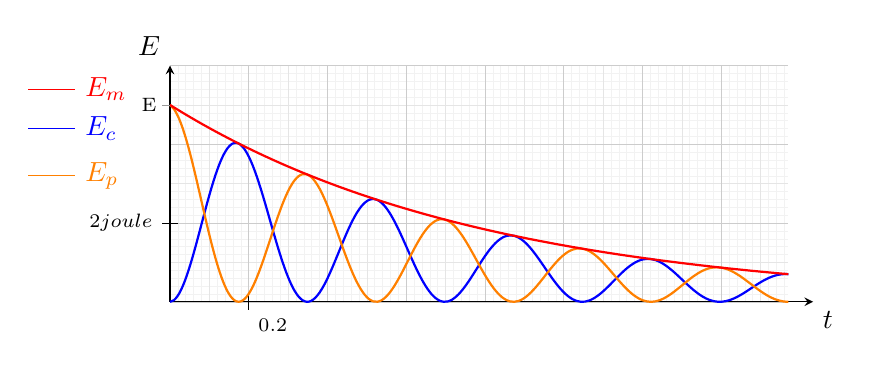
\begin{tikzpicture}[scale=1]
%papier milli
\draw [very thin, gray!10] (0,0) grid[step=0.1] (2.5*pi,3);
\draw [very thin, black!10] (0,0) grid[step=0.5] (2.5*pi,3);
\draw [very thin, black!20] (0,0) grid[step=1] (2.5*pi,3);
%fin

%axes
\draw[->,>=stealth] (0,0) -- (2.6*pi,0) node[below right] {$t$};
\draw[->,>=stealth] (0,0) -- (0,3) node [above left] {$E$};
\draw (1,0.1) -- (1,-0.1) node [below right] {{\scriptsize $0.2$}}; %échelle abscisse
\draw (0.1,1) -- (-0.1,1) node [left] {{\scriptsize $2joule$}}; %échelle ordonnée
%fin

%legend
\draw [red] (-1.8,2.7)--(-1.2,2.7) node [right] [red] {$E_m$};
\draw [blue] (-1.8,2.2)--(-1.2,2.2) node [right] [blue] {$E_c$};
\draw [orange] (-1.8,1.6)--(-1.2,1.6) node [right] [orange] {$E_p$};
%fin

\draw[color=blue,thick,domain=0:2.5*pi, samples=150,smooth] plot ({\x},{2.5*exp(-\x/4)*cos(1.8*\x r + pi/2 r)^2}); 
\draw[color=orange,thick,domain=0:2.5*pi, samples=150,smooth] plot ({\x},{2.5*exp(-\x/4)*sin(1.8*\x r + pi/2 r)^2});
\draw[color=red,thick,domain=0:2.5*pi, samples=150,smooth] plot ({\x},{2.5*exp(-\x/4)});
    

%\draw[color=gray,thin,dotted,domain=0:2.5*pi, samples=150,smooth] plot ({\x},{2.5*exp(-\x/4)});
%\draw[color=gray,thin,dotted,domain=0:2.5*pi, samples=150,smooth] plot ({\x},{-2.5*exp(-\x/4)});

%double flèche
%\draw[blue,line width=1pt,<->,>=triangle 45] (3.425,1.5) --++ (3.45,0) node [midway, below] {\colorbox{white}{\textcolor{blue}{\scriptsize{$T_\mathrm{\lambda = 1/4}$}}}} ;
%\draw[orange,line width=1pt,<->,>=triangle 45] (3.175,2.5) --++ (3.3,0) node [midway, above] {\colorbox{white}{\textcolor{orange}{\scriptsize{$T_\mathrm{\lambda = 1/2}$}}}} ;

%pointillés
%\draw [very thin,blue!80, dashed] (3.425,0) --++ (0,1.75) (6.9,0) --++ (0,1.75);
%\draw [very thin,orange!80, dashed] (3.175,0) --++ (0,2.75) (6.475,0) --++ (0,2.75);
\draw [very thin,gray!80, dashed] (-0.1,2.5) --++ (0.2,0) node [left=0.15cm, black] {\scriptsize{E}};
\end{tikzpicture}


\end{center}


\section{Etude énergétique d'un pendule de Torsion :}

\subsection{Energie cinétique du système: }
L'énergie cinétique du pendule de torsion est égale à l'énergie cinétique de la tige qui est donnée par l'expression suivante:
$E_c = \frac{1}{2}.J_\Delta.\dot{\theta}^2$

\subsection{Energie potentielle de torsion:}

L'énergie potentielle de torsion est donnée par la la relation suivante: $E_p = \frac{1}{2}.C.\theta^2 + C$

Cte: est une constante qui dépend du choix de l’état de référence de l’énergie potentielle de torsion .

En considérant comme état de référence $E_p = 0$ lorsque $\theta = 0$ $E_p = \frac{1}{2}C.\theta^2$ donc C=0

\subsection{Energie mécanique du pendule de torsion: }

L'énergie mécanique du pendule de torsion est la somme de son énergie cinétique et son énergie potentielle de torsion. $$E_m = E_c + E_p$$

En considérant comme état de référence E p t=0 lorsque $\theta = 0$, l'énergie mécanique du pendule de torsion s'écrit: 
$$E_m = \frac{1}{2}.J_\Delta.\dot{\theta}^2 + \frac{1}{2}.C.\theta^2$$

Si les frottements sont négligeables, l'énergie mécanique de l'oscillateur est constante 
$\frac{dE_m}{dt} = 0$ donc $E_m = Constante$

équation différentielle. $J_\Delta.\ddot{\theta} + C.\theta = 0$

\subsection{Diagramme énergétiques :}
En considérant comme état de référence E p t=0 lorsque $\theta = 0$ , la constante C=0 donc: $E_p = \frac{1}{2}.C.\theta^2$

\begin{center}
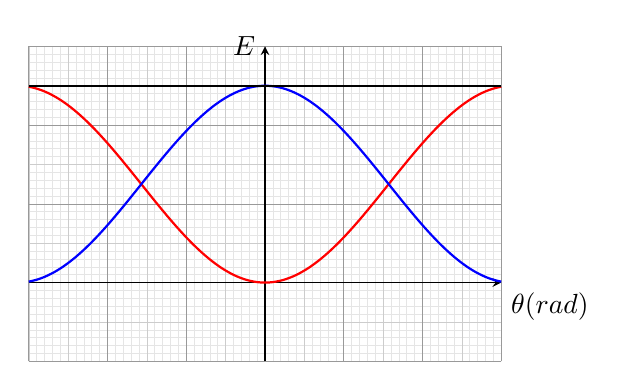
\begin{tikzpicture}[scale=1]
%papier milli
\draw [very thin, gray!20] (-3,-1) grid[step=0.1] (3,3);
\draw [very thin, black!20] (-3,-1) grid[step=0.5] (3,3);
\draw [very thin, black!40] (-3,-1) grid[step=1] (3,3);
%fin 
axes \draw[->,>=stealth] (-3,0) -- (3,0) node[below right] {$\theta(rad)$};
%stealth définit un style de flèche, "furtif"
\draw[->,>=stealth] (0,-1) -- (0,3) node[left] {$E$};
%\draw (1,0.1) -- (1,-0.1) node [below right] {{\scriptsize $0.2$}}; %échelle abscisse
%\draw (0.1,1) -- (-0.1,1) node [left] {{\scriptsize $2V$}}; %échelle ordonnée
%fin
%legende \draw (-2,3) -- (-0.4,3) -- (-0.4,1.9) -- (-2,1.9) -- (-2,3); %cadre
%\draw [red] (-1.8,2.7)--(-1.2,2.7) node [right] [red] {$E_p$};
%\draw [blue] (-1.8,2.2)--(-1.2,2.2) node [right] [blue] {$E_c$};
%fin
\draw[color=red,thick,domain=-3:3, samples=150] plot ({\x},{2.5*sin(0.5*\x r )^2});
\draw[color=blue,thick,domain=-3:3, samples=150] plot ({\x},{2.5*cos(0.5*\x r )^2});

\draw[color=black,thick,domain=-3:3, samples=150] plot ({\x},{2.5});
\end{tikzpicture}

\end{center}



\section{Etude énergétique du pendule pesant : }

\subsection{Energie cinétique du système:}
L'énergie cinétique du pendule pesant est: $E_c = \frac{1}{2}.J_\Delta.\dot{x}^2$

\begin{wrapfigure}{r}{0.2\textwidth}
	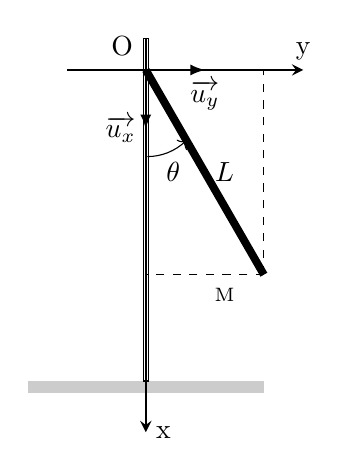
\begin{tikzpicture}[scale=1] 
	\fill [gray,opacity=0.4] (0,-0.5) rectangle (3,-0.35);
	\draw (1.47,-0.35) rectangle (1.53,4);
	
	\draw [->] (1.52,2.5) arc (-90:-45:0.7); 
	\node at (1.85,2.3) {$\theta$}; 
	
	
	%repère cartésien                                               
	\node at (1.2,3.9) {O};
	\draw [->,-stealth,thick] (0.5,3.6) --++ (3,0) node [above] {y};
	\draw [->,-latex,thick] (1.5,3.6) --++ (0.75,0) node [below] {$\overrightarrow{u_y}$};
	\draw [->,-stealth,thick] (1.5,4) --++ (0,-5) node [right] {x};
	\draw [->,-latex,thick] (1.5,3.6) --++ (0,-0.75) node [left] {$\overrightarrow{u_x}$};		              
	%fin

	\draw node at (2.5,2.3) {$L$}; 

	%\filldraw [black] (1.5,3.6) circle (0.08cm);
	\draw [black ,line width=0.1cm] (1.5,3.6) -- (3,1);
	%\draw [color=white,ball color=gray,smooth] (3,1) circle (0.2); 
	\node at (2.5,0.75) {\scriptsize{M}} ;
 
	
	
	 \draw [dashed] (3,1)--++(0,2.6);                                               
	 \draw [dashed] (3,1)--++(-1.5,0); 
	\label{pendule_base_polaire}	                                              
	\end{tikzpicture}

\end{wrapfigure}


\subsection{Energie potentielle de pesanteur:}
L'énergie potentielle de pesanteur du pendule pesant est : $E_{pp} = mgz + C$

En considérant comme état de référence E p p=0 lorsque z = 0 la constante C=0 donc $E_{pp} = mgz$

Lorsque le pendule pesant est incliné d'un angle $\theta$ , son énergie potentielle de pesanteur $E_{pp} = mgz_G$

avec $z_G = d- OH = d-dcos(\theta) = d(1-cos\theta)$ donc $$E_{pp}=mgd\big(1-cos(\theta)\big)$$

pour $\theta = -1$ l'énergie potentielle $E_{ppmax} = 2.m.g.d$

\underline{On a deux cas possibles : }
\begin{itemize}

	\item $E_m > 2.m.g.d$, l'énergie cinétique du système ne s'annule pas et le système se met à tourner sans arrêt et ce n'est pas un oscillateur mécanique.

	\item $E_m < 2.m.g.d$, l'énergie cinétique du système ne s'annule aux position $\theta = \ddag \theta_m$ 
et il oscille de façon périodique.
\end{itemize}

\subsection{Energie mécanique du pendule pesant: }
En considérant comme état de référence $E_{pp}=0$ lorsque z=0,  L'énergie mécanique du système : $E_m = E_c + E_{pp} = \frac{1}{2}.J_\Delta.\ddot{\theta}^2 + mgz$

\subsection{Diagramme énergétiques :}






Pour les petites oscillations $\theta \leq 15^{\circ}$ donc $cos(\theta) = 1- \frac{\theta^2}{2}$
on peut écrire par approximation $E_{pp} = \frac{m.g.d.\theta^2}{2}$ dans ce cas on a: 


%\begin{center}

	%\includegraphics[width=0.6\textwidth]{./img_02.png}
%\end{center}



%\begin{wrapfigure}{r}{0.3\textwidth}
	%\vspace{-2cm}
	%\includegraphics[width=0.3\textwidth]{./img_00.png}
%\end{wrapfigure}

\end{document}

